\chapter{結果與討論}
\label{ch:method}
在本研究中,我們利用密度泛函理論(Density functional theory, DFT),是以電子密度取代波函數作為研究的基本量的方法。利用DFT我們可以通過第一原理計算軟體進行自洽計算,獲得系統的本徵能量,從而瞭解材料的電子結構和響應性質。本研究將利用第一原理計算軟體Abinit中所提供的密度泛函理論的光學模組\cite{veithen2005nonlinear},包含以獨立粒子近似法為基礎的SHG光譜計算模組,進而計算二階極化率,定量地描述SHG響應。
% 3-1

% 隨著氮化鎵的應用日益多元,全面掌控氮化鎵的差排品質,對後續元件功能影響至為關鍵。目前,雖然市面上亦有其他可大量掃描差排密度的儀器,彈藥進一步深層分析氮化鎵的差排密度和類性,TEM雙束繞射丞相是目前唯一可以辨別差排類型的材料分析工具。本文簡單地介紹此分析技術,要進行足量的差排方溪已達到統計學上的要求,並歸納出差排類型和密度對元件品質的因果關係,仍需持續累積大量TEM影像拍攝和分析工作。這項工作雖然耗時,但是對於深入了解氮化鎵單晶的性質和影響因素,仍是非常重要的前瞻研究。
% \section{受應變影響的SHG特性}
\section{無缺陷的氮化鎵結構}
無缺陷的纖鋅礦氮化鎵(GaN)結構,其點群對稱性為$C_{6v}$,而此點群因不具有中心對稱性,因此GaN材料具有可產生SHG效應的條件。
我們先對無缺陷的GaN結構進行SHG模擬,可以得到
\begin{figure}
    \centering
    \includegraphics[width=1.0\linewidth]{Perfect_chi.png}
    \caption{(a)無缺陷的GaN以及在$xy$平面上的晶格向量。(b)為$C_{6v}$點群由Neumann principle推導出的二階極化率非零張量分布。黑色小點為零;有顏色的圓形為非零,顏色相同為值相同。(c)為經Abinit軟體模擬出的而階極化率張量絕對值。}
    \label{fig:defect-free}
\end{figure}

% \begin{figure}
%     \centering
%     \includegraphics[width=0.6\linewidth]{GaN_coordinate.png}
%     \caption{GaN晶體結構俯視圖。綠色表示為鎵原子,灰色表示為氮原子。x對應$[11\overline{2}0]$、y對應$[1\overline{1}00]$、z對應$[0001]方向。$}
%     \label{fig:GaN_coordinate}
% \end{figure}

\section{堆疊錯誤缺陷對SHG極化率張量的影響}
在氮化鎵晶體的成長過程中,除了理想的纖鋅礦(Wurtzite)結構外,常常伴隨著不同缺陷結構的產生,其中之一為堆疊錯誤(Stacking Fault, SF)。纖鋅礦結構的堆疊順序為ABABAB...,然而在實際成長過程中,可能會因為應變、雜質或介面效應而導致局部區域的堆疊方式改變,使得晶體出現與閃鋅礦結構(Zinc blende)類似的ABCABC...堆疊的片段,如圖~\ref{fig:SF_figure}所示。
% 具體的討論在氮化鎵晶體中的缺陷結構,我們由堆疊錯誤(Stacking fault)結構著手。前一章節有提到氮化鎵晶體具有兩種不同的堆疊方式,其中我們所研究的結構為較為穩定的纖鋅礦(wurtzite)結構,其結構堆疊的方式為ABABAB堆疊。而在實際氮化鎵晶體的生長過程中可能會有堆疊錯誤的產生,使晶體的局部區域出現類似閃鋅礦結構的堆疊方式,如圖~\ref{fig:SF_figure}所示。

根據文獻\cite{PhysRevB.71.235334, liliental2014structural},堆疊錯誤可以分為三種類型,差異主要是在局部的原子層排列的改變。我們利用可視化晶格結構的軟體VESTA\cite{momma2011vesta}建構出這三種堆疊錯誤的模型,如圖(~\ref{fig:SF_figure}),並進一步透過第一原理計算軟體模擬其SHG的二階極化率張量($\chi^{(2)}$)。透過比較缺陷結構與完美的纖鋅礦結構的的SHG響應,我們可以探討堆疊錯誤對材料非線性光學效應的影響。
% 如前一章節所述,堆疊錯誤可分為三種不同的形式,如圖~\ref{fig:SF_figure}。我們利用可視化晶格結構的軟體VESTA,建構出三種堆疊錯誤的模型,並進行對應的SHG模擬計算。

\begin{figure}[H]
    \centering
    \includegraphics[width=1.0\linewidth]{SF_figure_有背景.png}
    \caption{氮化鎵晶體堆疊錯誤類型\cite{PhysRevB.71.235334,liliental2014structural,komninou2005partial}。}
    \label{fig:SF_figure}
\end{figure}

% \begin{figure}[H]
%     \centering
%     \includegraphics[width=1.0\linewidth]{SF_data_有背景.png}
%     \caption{氮化鎵不同的堆疊錯誤缺陷類型的SHG模擬結果。在表格極化率張量欄位,其每個點的位置對應式,黑色的小點表示其值為零,紅色點表示該位置有值,實心連線表示為該連線的兩個張量元值相同,虛線連線表示為在Kleinman's symmetry成立的情況下有效。在表格中的最後一欄呈現的是不同的入射光能量對應的$\chi^{(2)}$的模擬結果圖。我們選擇能量為1.181eV(波長為1050nm)作為分析標準,取該能量下的極化率張量分量值進行比較與討論。}
%     \label{fig:SF_data.png}
% \end{figure}

\begin{figure}[H]
    \centering
    \includegraphics[width=1.1\linewidth]{SF_susceptibility_table.pdf}
    \caption{氮化鎵不同的堆疊錯誤缺陷類型的SHG模擬結果。極化率張量一欄是將模擬結果一欄的數值簡化表示:
    正方形表示為會影響$P_x$分量
    ;三角形表示為會影響$P_y$分量
    ;圓形表示為會影響$P_z$分量
    ;黑色的小點表示其值為零。顏色相同表示其絕對值相同。
    在表格最後一欄為第一原理模擬出的極化率張量$\chi^{(2)}$的絕對值。我們選擇能量為1.181eV(波長為1050nm)作為分析標準,取該能量下的極化率張量分量值進行比較與討論。}
    \label{fig:SF_table}
\end{figure}

如圖~\ref{fig:SF_table} 所示,氮化鎵中不同類型的堆疊錯層(Stacking Fault, SF)相較於無缺陷的結構有不同的點群對稱性。% 在原子排列、對稱性與非線性光學響應上皆展現出明顯差異。
無缺陷的結構具有六重對稱性,其點群為 $C_{6v}$,對應的二階極化率張量(Second-order susceptibility tensor)具有高對稱性的分量限制。然而,$I_1$ 與 $I_3$ 型堆疊錯誤破壞了六重對稱性,其點群降低為 $C_{3v}$,使得更多非零的張量分量出現。$I_2$ 型則雖然維持在 $C_{6v}$ 對稱性,但非零的張量元值會有改變。

\section{刃狀差排(Edge Dislocation)的應力分布}
實際氮化鎵材料中,刃狀差排(Edge Dislocation)的大小大約是微米等級,因此若是我們要建構實際大小的刃狀差排結構進行SHG模擬,所需要建立的超晶胞中可能需要包含幾千幾萬顆原子。而當實空間中的晶格向量變大時,其對應的倒空間的晶格向量將會變小,使得布里淵區的範圍縮小,刃狀差排會破壞晶體的平移對稱性,因此需要使用足夠大的超晶胞,才能夠有效捕捉刃狀差排造成晶體的局部改變對SHG的影響。

然而,隨著晶胞內的原子數量增加,進行第一原理計算所需要的資源與時間成本也會大幅提升,使得直接模擬大型的缺陷結構變得較為困難。為了降低計算成本,且同時能探討缺陷對SHG訊號的影響,我們透過了解刃狀差排對晶體造成的應力,來簡化SHG的模擬。
由於實際的刃狀差排尺寸較大,為了清楚呈現其對晶胞內原子位移的影響,我們先建立較小的超晶胞,並利用Atomsk軟體\cite{hirel2015atomsk},透過設定伯格向量(Burgers vector)$[11\overline{2}0]$,以及差排線(Dislocation line)$[0001]$建構出含有刃狀差排的GaN結構,如圖~\ref{fig:edge_dislocation_atomsk_displacement}中,紅色圓圈所標示的位置為刃狀差排的位置,也就是額外插入的一排原子;綠色透明的原子代表無缺陷的GaN結構;褐色的原子則代表含有刃狀差排的GaN結構。藍色箭頭表示當結構中存在刃狀差排時,原子的位移方向,而箭頭長度則對應位移的大小。可以觀察到,靠近刃狀差排核心的原子位移量較大,隨著距離中心逐漸增加,位移量也逐漸減小。
這樣的位移分布可以看到,在刃狀差排插入的區域,原子之間的距離縮短,因而形成局部的壓縮應變。
此圖可以幫助我們了解在完美的GaN結構中引入刃狀差排缺陷後,晶胞內的原子所產生的位移與晶格應變的現象。
並且此軟體可以利用解析的應力公式,式(~\ref{eq:edge_stress}),計算出含有刃狀差排結構的應力分布,如圖~\ref{fig:edge_stress}。
% 圖(~\ref{fig:edge_dislocation_atomsk})(a)為完美無缺陷的GaN結構,
% (b)則為含有刃狀差排的結構,其中紅色方框標示額外插入的一排原子。在完美晶格中,x方向共有九個六邊形,而在(b)含有刃狀差排的結構中,上半平面(藍色區域)在x方向多了一個六邊形。黑色直線表示完美結構中一個六邊形的間距;在(b)中,藍色與紅色箭頭分別表示原子向內與向外的位移,上半平面(藍色區域)表示此部分的原子位移為壓縮,下半平面(紅色區域)表示此部分的原子位移為往外拉伸。


\begin{figure}[H]
    \centering
    \includegraphics[width=1.0\linewidth]{figure_16.pdf}
    \caption{刃狀差排結構相對無缺陷結構的原子位移圖。利用Atomsk軟體\cite{hirel2015atomsk}設定刃狀差排的差排線(Dislocation line)$[0001]$,以及伯格斯向量(Burgers vector)$[11\overline{2}0]$生成GaN的刃狀差排結構。
    綠色透明的部分為完美的GaN結構;深紅色為含有刃狀差排的結構;紅色圓圈標示刃狀差排的位置;藍色箭頭為表示超晶胞中的原子因刃狀差排的插入而被向外推擠,產生的位移,箭頭方向表示位移方向,箭頭長度表示位移的大小。}
\label{fig:edge_dislocation_atomsk_displacement}
\end{figure}
%%%%%%%%%%%%%%%%%%%%%%%%%%%%%%%%%%%%%%%%%
%%應力
%\begin{figure}[H]
%    \centering
%    \includegraphics[width=1.0\linewidth]{50301_0.5_0.1_3.189_stress.pdf}
%    \caption{使用atomsk軟體將dislocation插入完美的晶格中,並可用解析的應力公式計算出應力的分布。紅色矩形標示的位置為刃狀差排。(a)為$\sigma_{xx}%$;(b)為$\sigma_{yy}$;(c)為$\sigma_{xy}$;(d)為$\sigma_{zz}$。}
%    \label{fig:edge_stress}
%\end{figure}

\begin{figure}[H]
    \centering
    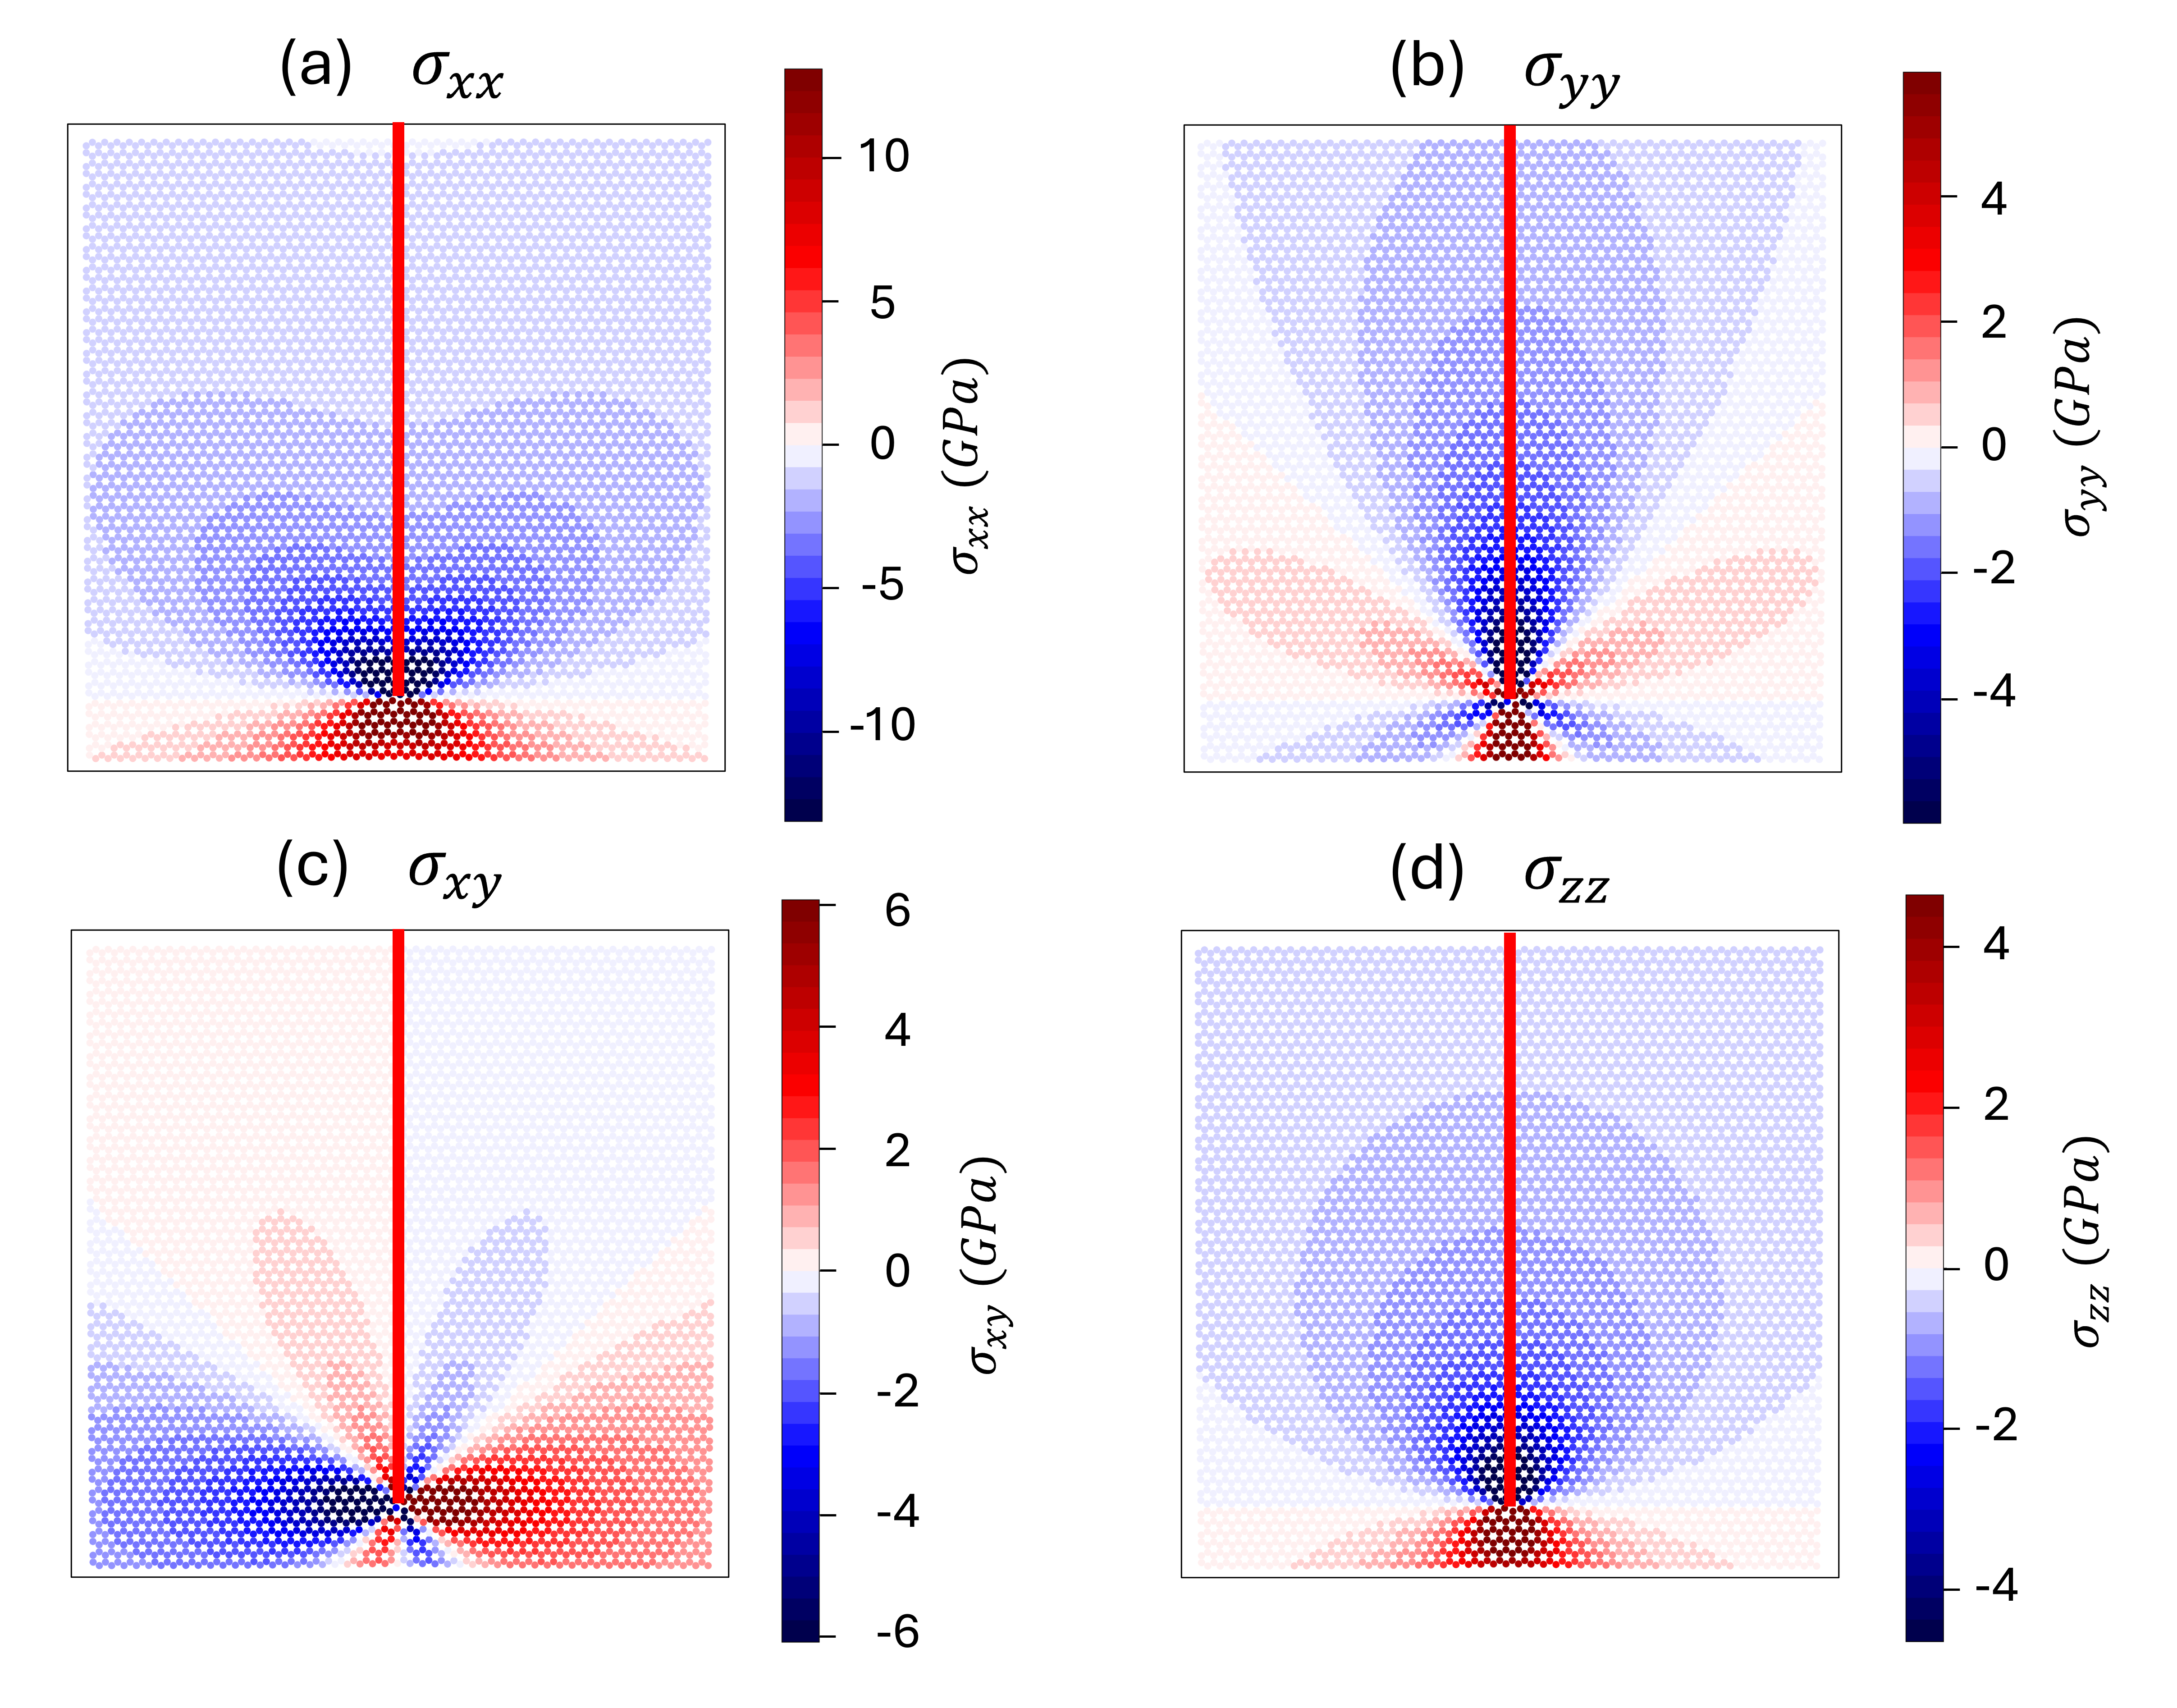
\includegraphics[width=1.0\linewidth]{stress_0904_new.png}
    \caption{使用atomsk軟體\cite{hirel2015atomsk}將刃狀差排插入完美的晶格中,並可用解析的應力公式計算出應力的分布。紅色矩形標示的位置為刃狀差排。(a)為$\sigma_{xx}$;(b)為$\sigma_{yy}$;(c)為$\sigma_{xy}$;(d)為$\sigma_{zz}$。}
    \label{fig:edge_stress}
\end{figure}

%%%%%%%%%%%%%%%%%%%%%%%%%%%%%%%%%%%%%%%%%

在圖~\ref{fig:stress_minus}(a)中,$\sigma_{xx}-\sigma_{yy}$顯示在$x$方向與$y$方向應力相減後的分布,可以觀察到整體應力值變化不大,顯示主要貢獻來自$x$方向的應力;在靠近差排的位置,應力趨近於零。而在圖~\ref{fig:stress_minus}(c)中,$\sigma_{xx}+\sigma_{yy}$對應於圖~\ref{fig:edge_stress}(a)與(b)的疊加結果,可見數值有所增加,但主要貢獻仍為$x$方向,而在差排附近,其數值大致落在$0$至$-5$的範圍內。綜合而言,在$xy$平面內,主要平面應力來自$x$方向,而在差排核心區域,雖然$x$與$y$方向的應力皆有貢獻,因此可將此區域視為有$x$方向與$y$方向的雙軸(Biaxial)壓應力。
此外,圖~\ref{fig:stress_minus}(b)為$\sigma_{xx}-\sigma_{zz}$,與圖~\ref{fig:edge_stress}中的(a)與(d)相比,可以看出應力仍主要集中在x方向;圖~\ref{fig:stress_minus}(d)顯示$\sigma_{xx}+\sigma_{zz}$,其數值確實進一步增加。
綜合圖~\ref{fig:stress_minus}的比較可知,
刃狀差排在在空間中主要引發的應力方向為$x$方向的單軸應力(Uniaxial stress),並且在差排插入附近的區域會形成壓應力(Compressive stress)。

\begin{figure}[H]
    \centering
    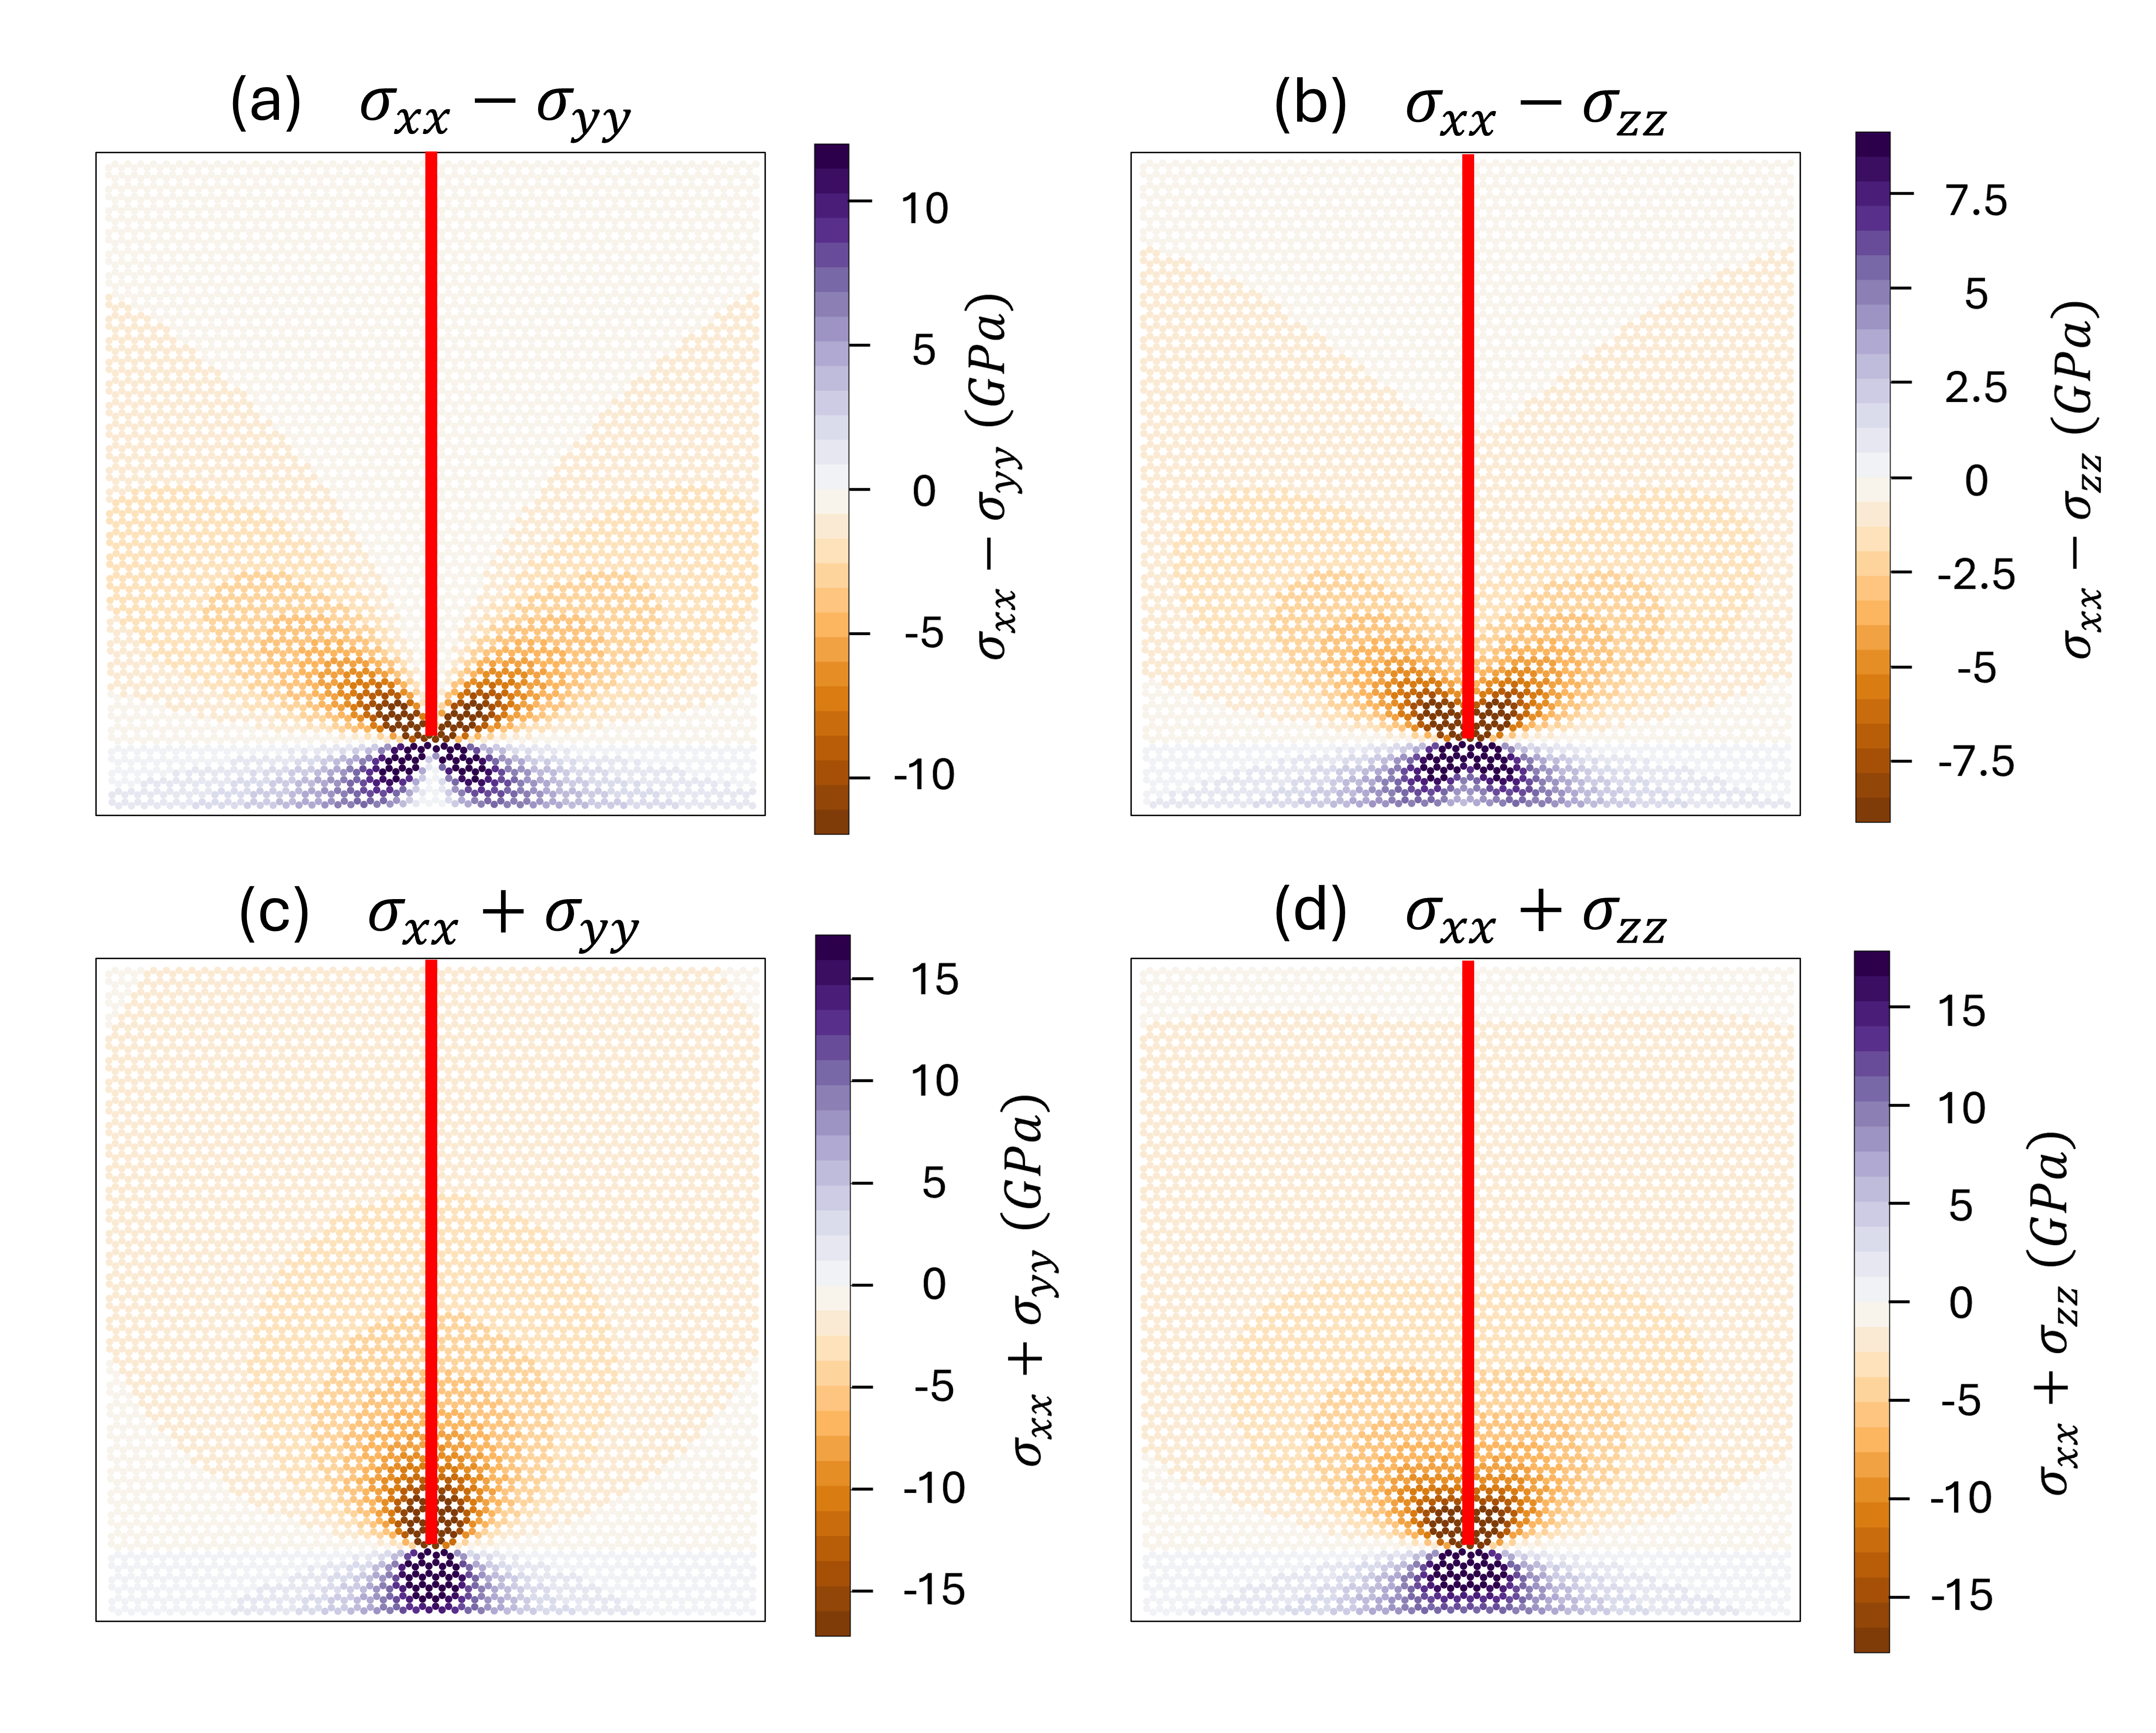
\includegraphics[width=1.0\linewidth]{stress_minus_0904.png}
    \caption{(a)為$\sigma_{xx}-\sigma_{yy}$。顯示在$x$方向與$y$方向應力相減後的分布,可以觀察到整體應力值變化不大,顯示主要貢獻來自$x$方向的應力。(c)為$\sigma_{xx}+\sigma_{yy}$對應於圖(~\ref{fig:edge_stress})(a)與(b)的疊加結果,可見數值有所增加,但主要貢獻仍為$x$方向,而在差排附近,其數值大致落在$0$至$-5$的範圍內。
    (b)為$\sigma_{xx}-\sigma_{zz}$,與圖(~\ref{fig:edge_stress})中的(a)與(d)相比,可以看出應力仍主要集中在x方向。(d)顯示$\sigma_{xx}+\sigma_{zz}$,其數值確實進一步增加,但主要貢獻還是在x方向。綜合比較可知,刃狀差排在在空間中主要引發的應力方向為x方向,並且在差排插入附近的區域會形成壓應力(Compressive stress)。}
    \label{fig:stress_minus}
\end{figure}

%------------------------------------------------------------------------------------------

\subsection{應變與SHG張量的變化分析}
本研究中是將應力轉變為應變後,利用應變張量對晶體結構作用,且不進行鬆弛計算(relaxation),觀察在晶體中施加應力對其SHG響應的影響。
應力-應變轉換公式\cite{de2015charting}
\begin{equation}
    \begin{pmatrix}
        \sigma_{xx} \\ \sigma_{yy} \\ \sigma_{zz} \\ \sigma_{yz} \\ \sigma_{xz} \\ \sigma_{xy}
    \end{pmatrix}
    =\begin{pmatrix}
        C_{11} & C_{12} & C_{13} & 0 & 0 & 0 \\
        C_{12} & C_{11} & C_{13} & 0 & 0 & 0 \\
        C_{13} & C_{13} & C_{33} & 0 & 0 & 0 \\
        0 & 0 & 0 & C_{44} & 0 & 0 \\
        0 & 0 & 0 & 0 & C_{44} & 0 \\
        0 & 0 & 0 & 0 & 0 & C_{66}
    \end{pmatrix}
    \begin{pmatrix}
        \varepsilon_{xx} \\ \varepsilon_{yy} \\ \varepsilon_{zz} \\ 2\varepsilon_{yz} \\ 2\varepsilon_{xz} \\ 2\varepsilon_{xy}
    \end{pmatrix}
\end{equation}
其中$C_{ij}$是彈性係數,GaN的彈性係數為$C_{11}=390$GPa,$C_{12}=145$GPa,$C_{13}=106$GPa,$C_{33}=398$GPa,$C_{44}=105$GPa,$C_{66}=122.5$GPa\cite{vurgaftman2003band}\cite{polian1996elastic}。若是要將應力轉換成應變,可利用彈性常數矩陣的反矩陣進行轉換
\begin{equation}
    \varepsilon_i=\sum_{j=1}^6 S_{ij}\sigma_j
    \label{eq:strain_to_stress}
\end{equation}
其中$i,j=1,2,...,6$,對應的分量為,$1=xx,2=yy,3=zz,4=yz,5=xz,6=xy$。
藉由式(~\ref{eq:strain_to_stress})可以將計算出的edge dislocation的應力場轉為應變,再將應變場作用在晶體結構中。

藉由前一小節得知,刃狀差排的插入會使得晶體有$x$方向的單軸應變(Unaxial strain)以及在$x$、$y$方向的雙軸應變(Biaxial strain),因此我們利用對晶體施加應變使其對稱性改變,且不進行鬆弛計算(relaxation),並利用Abinit軟體進行二階極化張量(Second-order susceptibility tensor)計算。我們先對GaN材料施加單軸應變,沿著$x$方向($[11\overline{2}0]$)施加$\pm 0.01$的應變量(對應於1\%的拉伸或壓縮),如圖~\ref{fig:defect-free}(a),利用式~\ref{eq:uniaxial_strain}對晶體進行x方向的單軸應變。
\begin{equation}
\varepsilon=
    \begin{pmatrix}
        \pm 0.01 & 0 & 0\\
        0 & 0 & 0 \\
        0 & 0 & 0 
    \end{pmatrix}
    \label{eq:uniaxial_strain}
\end{equation}
以及針對$x$、$y$軸進行雙軸施加$\pm 0.01$的應變量,如式~\ref{eq:biaxial_strain},並將應變後的晶格結構進行SHG效應的模擬分析。   %要記得確認數字跟數據
\begin{equation}
\varepsilon=
    \begin{pmatrix}
        \pm 0.01 & 0 & 0 \\
         0 & \pm 0.01 & 0 \\
         0 & 0 & 0
    \end{pmatrix}
    \label{eq:biaxial_strain}
\end{equation}


\begin{figure}[H]
    \centering
    \includegraphics[width=1.0\linewidth]{strain_susceptibility_figure.png}
    \caption{對氮化鎵晶體作單軸應變,並模擬其二階極化率張量值。極化率張量一欄是將模擬解果一欄的數值簡化表示:正方形表示為會影響$P_x$分量;三角形表示為會影響$P_y$分量;圓形表示為會影響$P_z$分量;黑色的小點表示其值為零。顏色相同表示其絕對值相同。在表格最後一欄為第一原理模擬出的極化率張量$\chi^{(2)}$的絕對值。}
    \label{fig:strain0.01_table}
\end{figure}

%------------------------------------------------------------------------------------------

\section{SHG強度分析}

\subsection{極化向量與SHG強度計算}
在本節中,我們探討不同晶體結構在各種入射與偏振條件下的SHG強度分布。根據前述理論推導,SHG強度與入射光的偏振方向、入射角度$\theta$及方位角$\phi$密切相關。

入射光的行進方向$\hat{\mathbf{q}}$與偏振基底向量$\hat{\boldsymbol{\varepsilon}}_{P}$與$\hat{\boldsymbol{\varepsilon}}_{S}$分別為:
\begin{align}
    & \hat{\mathbf{q}} = \sin\theta(\cos\phi\, \hat{x} + \sin\phi\, \hat{y}) + \cos\theta\, \hat{z} \\
    & \hat{\boldsymbol{\varepsilon}}_{P} = \cos\theta(\cos\phi\, \hat{x} + \sin\phi\, \hat{y}) - \sin\theta\, \hat{z} \\
    & \hat{\boldsymbol{\varepsilon}}_{S} = -\sin\phi\, \hat{x} + \cos\phi\, \hat{y}
\end{align}
其中,$\hat{\boldsymbol{\varepsilon}}_{P}$表示在入射面內的偏振(P偏振),$\hat{\boldsymbol{\varepsilon}}_{S}$為垂直於入射面的偏振(S偏振)。

分別假設入射光的偏振為$S$偏振與$P$偏振,並將$S$、$P$偏振的單位向量帶入式(~\ref{eq:chi_tensor})可以得到不同入射偏振所對應的極化向量$P_{P}$及$P_{S}$。
將極化向量代入SHG強度的計算公式:
\begin{equation}
    I_{\lambda\lambda'} \propto \left| \hat{\boldsymbol{\varepsilon}}_{\lambda'} \cdot \mathbf{P}_{\lambda}(2\omega) \right|^2
\label{eq:intensity}
\end{equation}
其中$\lambda$與$\lambda'$分別代表入射與出射光的偏振方向,若皆為P偏振,則為$I_{PP}$。


\subsection{堆疊錯誤缺陷的SHG訊號強度分析}
三種堆疊錯誤缺陷結構的點群對稱性分別為:
\begin{table}[h!]
    \centering
    \begin{tabular}{|>{\centering\arraybackslash}p{6cm}|>{\centering\arraybackslash}p{6cm}|}
    \hline
      \textbf{Type} & \textbf{Point group}\\
    \hline
        Perfect & $C_{6v}$ \\
    \hline
       $I_1\ type$  & $C_{3v}$ \\
    \hline
       $I_2 \ type$ &  $C_{6v}$ \\
    \hline
       $I_3\ type$  &  $C_{3v}$ \\
    \hline
    \end{tabular}
    \caption{堆疊錯誤結構的點群對稱性}
    \label{tab:placeholder}
\end{table}
藉由知道不同缺陷結構的點群對稱性,我們可以推得對應的極化率張量中的非零元。無缺陷的GaN與$I_2\ type$的堆疊錯誤結構的點群對稱性為$C_{6v}$,其非零的二階極化率張量元如下:
\begin{equation}
    \chi_{ijk}^{(2)} = 
    \begin{pmatrix}
        0 & 0 & 0 & 0 & \chi_{xxz}^{(2)} & 0 \\
        0 & 0 & 0 & \chi_{yyz}^{(2)} & 0 & 0 \\
        \chi_{zxx}^{(2)} & \chi_{zyy}^{(2)} & \chi_{zzz}^{(2)} & 0 & 0 & 0 
    \end{pmatrix}
\label{eq:c6v_tensor}
\end{equation}
其中滿足$\chi_{xxz}^{(2)} = \chi_{yyz}^{(2)}$,$\chi_{zxx}^{(2)} = \chi_{zyy}^{(2)}$。
分別將入射偏振為$S$、$P$的極化向量寫為:
\begin{align}
    \mathbf{P}_{P}(2\omega) =
    & -\epsilon_0 \chi_{xxz}^{(2)} \cos\phi \sin(2\theta)\, \hat{x} 
    - \epsilon_0 \chi_{xxz}^{(2)} \sin\phi \sin(2\theta)\, \hat{y} \notag \\
    & + \epsilon_0 \left( 
        \chi_{zxx}^{(2)} \cos^2\theta \cos^2\phi 
        + \chi_{zzz}^{(2)} \sin^2\theta 
    \right) \hat{z}
\end{align}
\begin{equation}
    \mathbf{P}_{S}(2\omega)=( \epsilon_0\chi_{zxx}^{(2)})\hat{z}
\end{equation}
依照式(~\ref{eq:intensity})可計算對應的SHG強度可寫為:
\begin{align}
    &  I_{PP} \propto\ 
    \Big| -\epsilon_0 \big( 
    \chi_{xxz}^{(2)} \sin(2\theta) \cos\theta 
     + \chi_{zxx}^{(2)} \cos^2\theta \sin\theta 
    + \chi_{zzz}^{(2)} \sin^3\theta \big) \Big|^2 \\ 
    & I_{PS} \propto\  
    \Big| \epsilon_0 \big( 
    \chi_{xxz}^{(2)} \sin(2\theta) \cos\phi \sin\phi 
    - \chi_{yyz}^{(2)} \sin(2\theta) \cos\phi \sin\phi \big)  \Big|^2 =0 \\
    & I_{SP} \propto \Big| -\epsilon_0\chi_{zxx}^{(2)}\sin{\theta}\Big|^2 \\
    & I_{SS} \propto 0
\end{align}

而$I_1、I_3\ type$的堆疊錯誤結構的點群對稱為$C_{3v}$,其對應的二階極化率張量:
\begin{equation}
    \chi_{ijk}^{(2)} = 
    \begin{pmatrix}
        0 & 0 & 0 & 0 & \chi_{xxz}^{(2)} & \chi_{xxy}^{(2)} \\
        \chi_{yxx}^{(2)} & \chi_{yyy}^{(2)} & 0 & \chi_{yyz}^{(2)} & 0 & 0 \\
        \chi_{zxx}^{(2)} & \chi_{zyy}^{(2)} & \chi_{zzz}^{(2)} & 0 & 0 & 0 
    \end{pmatrix}
    \label{eq:c3v_tensor}
\end{equation}
其中$\chi_{xxz}^{(2)} = \chi_{yyz}^{(2)}$,$\chi_{zxx}^{(2)} = \chi_{zyy}^{(2)}$,$\chi_{xxy}^{(2)} = \chi_{yxx}^{(2)} = -\chi_{yyy}^{(2)}$。
分別將入射偏振為$S$、$P$的極化向量寫為:
\begin{align}
    \mathbf{P}_{P}(2\omega) =
    & \left[-\epsilon_0 \chi_{xxz}^{(2)} \cos\phi \sin(2\theta) - \epsilon_0 \chi^{(2)}_{yyy}\cos^2{\theta}\sin({2\phi})\right]\, \hat{x} \notag \\
    + & \left[-\epsilon_0 \chi^{(2)}_{yyy}\cos^2{\theta}\cos{2\phi}-\epsilon_0 \chi_{xxz}^{(2)} \sin\phi \sin(2\theta)\right]\, \hat{y} \notag \\
    +& \left[ \epsilon_0 \chi_{zxx}^{(2)} \cos^2\theta + \chi_{zzz}^{(2)} \sin^2\theta 
    \right]\, \hat{z}
\end{align}
\begin{equation}
    \mathbf{P}_{S}(2\omega)=\epsilon_0\chi^{(2)}_{yyy}\sin({2\phi})\, \hat{x}+\epsilon_0\chi^{(2)}_{yyy}\cos({2\phi})\, \hat{y}+\epsilon_0\chi_{zxx}^{(2)}\sin^2{\phi}\, \hat{z}
\end{equation}
可計算出對應的SHG強度:
\begin{align}
    & I_{PP} \propto \Big\vert -\epsilon_0(\chi_{xxz}^{(2)}\sin{(2\theta})\cos{\theta}+\chi_{yyy}^{(2)}\cos^3{\theta}\sin{(3\phi)} \notag \\ & \quad \quad \quad+\chi_{zxx}^{(2)}\cos^2{\theta}\sin{\theta}+\chi_{zzz}^{(2)}\sin^3{\theta})\Big\vert ^2 \\
    & I_{PS} \propto \Big \vert -\epsilon_0\chi^{(2)}_{yyy} \cos{(3\phi)}cos^2{\theta}\Big\vert ^2 \\
    & I_{SP} \propto \Big \vert \epsilon_0(\chi_{yyy}^{(2)}\cos{\theta}\sin{(3\phi)}-\epsilon_0\chi_{zxx}^{(2)}\sin{\theta})\Big\vert ^2 \\
    & I_{SS} \propto \Big\vert \epsilon_0\chi_{yyy}^{(2)}\cos{(3\phi)}\Big\vert^2
\end{align}

%%%%分垂直入射跟斜向入射%%%%%%%%%%%%%%%%%%%%%%%%%%%%%%%%%%%%%%%%%
\subsubsection{當入射光為垂直入射}
我們已知不同點群對稱性所計算出的SHG強度與角度的關係,我們可以將入射光分為垂直入射與斜向入射進行討論,觀察SHG訊號強度與角度的關係。
首先我們假設入射光為垂直入射$\theta=0^\circ$,我們可以得到$C_{6v}$與$C_{3v}$點群分別對應的SHG強度為:
\begin{figure}[H]
    \centering
    \includegraphics[width=1.0\linewidth]{SF_I_phi_table.png}
    \caption{當入射光為垂直入射$\theta=0^\circ$,不同點群對應的SHG強度與方位角$\phi$的關係。}
    \label{fig:placeholder}
\end{figure}

可以得到SHG訊號強度與方位角$\phi$之間的關係,並畫出分布圖,圖~\ref{fig:Intensity_SF}。
在圖中可以看到只有點群為$C_{3v}$的結構($I_1$、$I_3\ type$)的SHG訊號強度會與方位角的變化有關,因為在入射光為垂直入射時,極化向量會包含x、y、z三個方向的分量,因此當收光方向在z方向,因此只探測$xy$平面上的偏振時,使可以接收到SHG訊號的,並可以將其強度與方位角的關係畫出,如圖~\ref{fig:Intensity_SF}中$\theta=0^\circ$一欄的橘色與綠色線。
而點群為$C_{6v}$的無缺陷結構以及$I_2\ type$的堆疊錯誤在入射光為垂直入射的情況下,因為極化率張量的非零值的分布使得極化向量只會有z方向的分量,因此當收光方向是在z方向時,是不會接收到SHG訊號的,便不會有SHG訊號強度與方位角的分布。


\subsubsection{當入射光為斜向入射}
當入射光為斜向入射,並我們假設入射光在$xz$平面$\phi=0^\circ$,我們可以得到$C_{6v}$與$C_{3v}$點群分別對應的SHG強度為:
\begin{figure}[H]
    \centering
    \includegraphics[width=1.1\linewidth]{SF_I_theta_table.png}
    
    \caption{當入射光為在$xz$平面上斜向入射$\phi=0^\circ$,不同點群對應的SHG強度與$\theta$的關係。}
    \label{fig:SF_theta}
\end{figure}
可以由此表格中的$\theta$與SHG強度的關係,畫出強度與角度的分布圖,圖~\ref{fig:Intensity_SF}。%%%%%%%%%%%
由於P偏振向量$\hat{\boldsymbol{\varepsilon}}_{P} = \cos\theta(\cos\phi\, \hat{x} + \sin\phi\, \hat{y}) - \sin\theta\, \hat{z}$是含有z方向的分量,因此當我們在收光端選擇P偏振時,便可以探測到極化向量的$z$方向分量。這一特性在圖~\ref{fig:Intensity_SF}中的$I_{PP}(\theta)$、$I_{SP}(\theta)$的分布圖中表現的較為明顯:因極化向量含有z分量,因此所產生的SHG主要是沿著平行樣品的表面的方向輻射,因此SHG強度會集中在平行樣品(靠近$90^{\circ}$)的區域。
相對地,S偏振向量$\hat{\boldsymbol{\varepsilon}}_{S} = -\sin\phi\, \hat{x} + \cos\phi\, \hat{y}$僅有$x$、$y$分量,因此在$I_{PS}(\theta)$與$\theta$角的分布圖中,強度多集中在垂直樣品方向,在平行方向上幾乎無訊號。

進一步觀察 $I_{PP}(\theta)$ 的分布圖,可以清楚看出堆疊錯誤缺陷結構與完美結構之間的 SHG 強度差異。由於缺陷導致晶體點群改變,進而改變極化率張量的形式(式(~\ref{eq:c3v_tensor})、式(~\ref{eq:c6v_tensor})),因此 SHG 強度的角度分布也隨之改變。以 $I_3$ 型堆疊錯誤為例,其 SHG 強度(綠色線)在 $30^\circ \sim 60^\circ$ 之間達到最大值;而完美結構(藍色線)則主要集中在接近 $90^\circ$ 的方向。這顯示缺陷不僅會改變SHG的總強度,也會改變其輻射方向性,反映出晶體對稱性與非線性響應間的關係。


% \begin{figure}[H]
%     \centering
%     \includegraphics[width=0.8\linewidth]{I_SF_theta_line.png}
%     \caption{堆疊錯誤缺陷結構與無缺陷的GaN結構的SHG訊號強度隨$\theta$角的變化,$\theta\in [-\frac{\pi}{2}, \frac{\pi}{2}]$。}
%     \label{fig:placeholder}
% \end{figure}

%\begin{figure}[H]
%    \centering
%    \includegraphics[width=1.0\linewidth]{SF_intensity.png}
%    \caption{堆疊錯誤結構的SHG強度與$\phi$、$\theta$角度的關係。當$\theta=0^\circ$,$\phi \in [0,2\pi]$;當$\phi=0^\circ$,$\theta \in %[-\frac{\pi}{2},\frac{\pi}{2}]$。}
%    \label{fig:Intensity_SF}
%\end{figure}

\begin{figure}[H]
    \centering
    \includegraphics[width=1.0\linewidth]{SF_intensity_0831.pdf}
    \caption{堆疊錯誤結構的SHG強度與$\phi$、$\theta$角度的關係。當$\theta=0^\circ$,$\phi \in [0,2\pi]$;當$\phi=0^\circ$,$\theta \in [-\frac{\pi}{2},\frac{\pi}{2}]$。}
    \label{fig:Intensity_SF}
\end{figure}

%%%%%%%%%%%%%%%%%%%%%%%%%%%%%%%%%%%

\subsection{應變結構的SHG訊號強度分析}
在單軸與雙軸應變的結構中,可以看到只有單軸應變會改變結構的點群對稱,而雙軸應變不會改變結構的點群對稱。依照單軸應變結構的點群對稱$C_{2v}$的極化率張量非零值的分布:
\begin{equation}
    \chi_{ijk}^{(2)} = 
    \begin{pmatrix}
        0 & 0 & 0 & 0 & \chi_{xxz}^{(2)} & 0 \\
        0 & 0 & 0 & \chi_{yyz}^{(2)} & 0 & 0 \\
        \chi_{zxx}^{(2)} & \chi_{zyy}^{(2)} & \chi_{zzz}^{(2)} & 0 & 0 & 0 
    \end{pmatrix}
\label{eq:c2v_tensor}
\end{equation}
且五個非零值皆不相同。分別將入射偏振為$S$、$P$的極化向量寫為:
\begin{align}
    \mathbf{P}_{P}(2\omega) =
    & -\epsilon_0 \chi_{xxz}^{(2)} \cos\phi \sin(2\theta)\, \hat{x} 
    - \epsilon_0 \chi_{yyz}^{(2)} \sin\phi \sin(2\theta)\, \hat{y} \notag \\
    & + \epsilon_0 \left( 
        \chi_{zxx}^{(2)} \cos^2\theta \cos^2\phi +\chi^{(2)}_{zyy}\cos^2{\theta}\sin^2{\phi} 
        + \chi_{zzz}^{(2)} \sin^2\theta 
    \right) \hat{z}
    \label{eq:C2v_P_P}
\end{align}
\begin{equation}
    \mathbf{P}_{S}(2\omega)=\epsilon_0(\chi_{zxx}^{(2)}\sin^2{\phi}+\chi^{(2)}_{zyy}\cos^2{\phi})\hat{z}
    \label{eq:C2v_P_S}
\end{equation}
可計算出對應的SHG強度:
\begin{align}
    & I_{PP} \propto \Big\vert -\epsilon_0(\chi_{xxz}^{(2)}\sin{(2\theta})\cos{\theta}\cos^2{\phi}+\chi_{yyz}^{(2)}\sin{(2\theta})\cos{\theta}\sin^2{\phi} \notag \\ & \quad \quad \quad+\chi_{zxx}^{(2)}\cos^2{\theta}\sin{\theta}\cos^2{\phi}+\chi^{(2)}_{zyy}\cos^2{\theta}\sin{\theta}\sin^2{\phi}+\chi_{zzz}^{(2)}\sin^3{\theta})\Big\vert ^2 \\
    & I_{PS} \propto \Big \vert -\epsilon_0(\chi^{(2)}_{xxz} \sin{(2\theta)}\cos{\phi}\sin{\phi}+\chi^{(2)}_{yyz}\sin{(2\theta)}\sin{\phi}\cos{\phi})\Big\vert ^2 \\
    & I_{SP} \propto \Big \vert -\epsilon_0(\chi_{zxx}^{(2)}\sin{\theta}\sin^2{\phi}+\chi_{zyy}^{(2)}\sin{\theta}\cos^2{\phi})\Big\vert ^2 \\
    & I_{SS} \propto 0
\end{align}

\subsubsection{當入射光為垂直入射}
當入射光以及收光方向皆為垂直樣品$\theta=0^\circ$時,由式~\ref{eq:C2v_P_P}以及式~\ref{eq:C2v_P_S}可以得知極化向量只剩下z分量存在,而垂直出射的光其偏振只會在$xy$平面上,因此不管是觀察S偏振或是P偏振的收光,皆不會有SHG訊號。
因此可以看到圖(~\ref{fig:strain_Intensity_table})中不管是有沒有施加應變的結構,在不同的入射及收光偏振下,其SHG強度皆為零。
\begin{figure}[H]
    \centering
    \includegraphics[width=1.0\linewidth]{I_strain_phi.png}
    \caption{無缺陷GaN以及應變結構的點群當$\theta=0^\circ$時,所對應的SHG強度與$\phi$角度的關係,$\phi \in [0 , 2\pi]$}
    \label{fig:strain_Intensity_table}
\end{figure}

\subsubsection{當入射光為斜向入射}
當假設入射光在$xz$平面$\phi=0^\circ$時,極化向量的分量主要分布在x與z方向。可以由圖~\ref{fig:Intensity_uniaxial_strain}看到,在x方向單軸應變的結構,其SHG訊號的強度主要分布在靠近樣品的區域,意味著其二階極化向量主要是在z方向,因此其幅射出的光強度為在平行樣品的方向。可以看到在圖~\ref{fig:Intensity_uniaxial_strain}中當入射光偏振不同(分別為P和S偏振)且收光偏振都相同為P偏振時,會改變其SHG訊號的強度,且拉伸與壓縮應變的強度也會有所改變。當入射光為P偏振時,壓縮應變的SHG強度大於拉伸應變;當入射光為S偏振時,拉伸應變的SHG強度大於壓縮應變。雖然不管是拉伸或是壓縮的單軸應變,其SHG訊號的強度相較於無缺陷的結構皆較微弱,但是在$x$方向上不同的應變還是會改變SHG訊號的強度。

\begin{figure}[H]
    \centering
    \includegraphics[width=1.0\linewidth]{I_strain_theta.png}
    \caption{無缺陷GaN以及應變結構的點群當$\phi=0^\circ$時,所對應的SHG強度與$\theta$角度的關係,$\theta \in [-\frac{\pi}{2} , \frac{\pi}{2}]$}
    \label{fig:placeholder}
\end{figure}

\begin{figure}[H]
    \centering
    \includegraphics[width=1.0\linewidth]{uniaxial_intensity.png}
    \caption{當$\phi=0^\circ$,入射光與出射光皆在$xz$平面,單軸應變結構與於缺陷結構的SHG強度與$\theta$角度的關係比較。}
    \label{fig:Intensity_uniaxial_strain}
\end{figure}
在雙軸應變的結構中,因雙軸應變不會改變結構的點群對稱性,因此其極化率張量的非零值分布以及滿足的形式皆與無應變的GaN結構相同,皆為$C_{6v}$。但可以從圖(~\ref{fig:Intensity_biaxial_strain})中看到,在入射光為P偏振的情況下,雙軸拉伸應變結構的SHG強度明顯大於無缺陷結構,而雙軸壓縮應變相較於無缺陷結構較小;在入射光為S偏振時,拉伸與壓縮的雙軸應變結構SHG強度皆較無缺陷結構弱。可以明顯看到入射光的偏振對於SHG強度的影響程度,入射S偏振的光,其SHG結構皆會較入射P偏振光的強度弱。
\begin{figure}[H]
    \centering
    \includegraphics[width=1.0\linewidth]{biaxial_intensity.png}
    \caption{當$\phi=0^\circ$,入射光與出射光皆在$xz$平面,雙軸應變結構與於缺陷結構的SHG強度與$\theta$角度的關係比較。}
    \label{fig:Intensity_biaxial_strain}
\end{figure}